\documentclass[]{article}
\usepackage{graphicx}
\usepackage{float}


\graphicspath{{./images/}}
\usepackage[spanish]{babel}
\usepackage{url}
\usepackage{booktabs}
\usepackage{natbib}
%opening
\title{Framework Joyeuse}
\author{Jos\'e \'Angel Vald\'ez Torres, Kevin Pe\~na Mora, Yael Atletl Bueno Rojas}


\begin{document}

\maketitle

\begin{abstract}
Framework para crear juegos 3d cuya mec\'anica principal sean los disparos, orientado al rango desde desarrolladores reci\'en iniciados o por iniciarse en el \'ambito, hasta aquellos con conocimiento avanzado. Se compone de una serie de editores entre los cuales se encuentran:
\begin{itemize}
	\item Personajes: Usando una interf\'az simple que permita unificar Inteligencia Artificial, Modelos, animaciones y sonidos. 
	\item Inteligencia Artificial: Mediante un \'arbol de comportamiento.
	\item Niveles: Interf\'az que permita dise\~nar niveles estilo BSP utilizando CSG, evitando as\'i los inconvenientes del alg\'oritmo BSP, pero manteniendo la facilidad de dise\~no que provee. 
	\item Scripts: Mediante un editor ASCII o visual, a elecci\'on del usuario, con la posibilidad de combinar ambos tipos de scripts. 
	
\end{itemize}

\end{abstract}
\newpage
\tableofcontents
\listoffigures
\newpage
\section{La organizaci\'on}


\subsection{Misi\'on}
Proveer herramientas que faciliten la creaci\'on de v\'ideo juegos, para acercar a personas sin conocimientos de programación al desarrollo de v\'ideo juegos, ya sean artistas, estudiantes, profesores o aficionados. Todo esto, buscando diversificar la industria de los v\'ideo juegos y aumentar el conocimiento de programaci\'on en la sociedad al ofrecer una introducci\'on amena, intuitiva y que acerque al usuario paulatinamente.



\subsection{Visi\'on} 
Ser el est\'andar global para el desarrollo de v\'ideo juegos, solicitado tanto por usuarios novatos como grandes empresas, jugando un papel importante en la construcci\'on del futuro de la industria. 


\subsection{An\'alisis: Fortalezas, Oportunidades, Debilidades, Amenazas}

\subsubsection{Organizacional}
\begin{figure}[H]
	
	\centering
	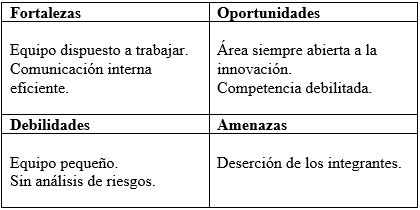
\includegraphics[width=0.6\textwidth]{org}
	\caption{Anal\'isis FODA de la organizaci\'on}
	
\end{figure}


\subsubsection{Jos\'e \'Angle Vald\'ez Torres }
\begin{figure}[H]
	
	\centering
	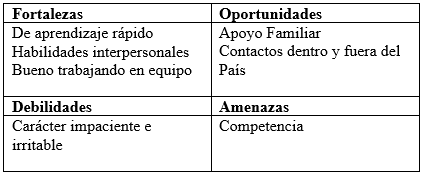
\includegraphics[width=0.6\textwidth]{jose}
	\caption{Anal\'isis FODA: Jos\'e \'Angel}
	
\end{figure}
\subsubsection{Kevin Pe\~na Mora}
\begin{figure}[H]
	
	\centering
	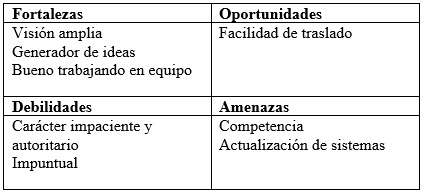
\includegraphics[width=0.6\textwidth]{kevin}
	\caption{Anal\'isis FODA: Kevin}
	
\end{figure}

\subsubsection{Yael Atletl Bueno Rojas}

\begin{figure}[H]
	
	\centering
	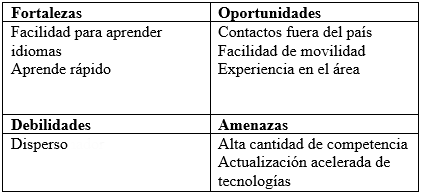
\includegraphics[width=0.6\textwidth]{yael}
	\caption{Anal\'isis FODA: Yael Atletl}
	
\end{figure}

\subsection{Estructura de Desglose de Trabajo}
\begin{figure}[H]
	
	\centering
	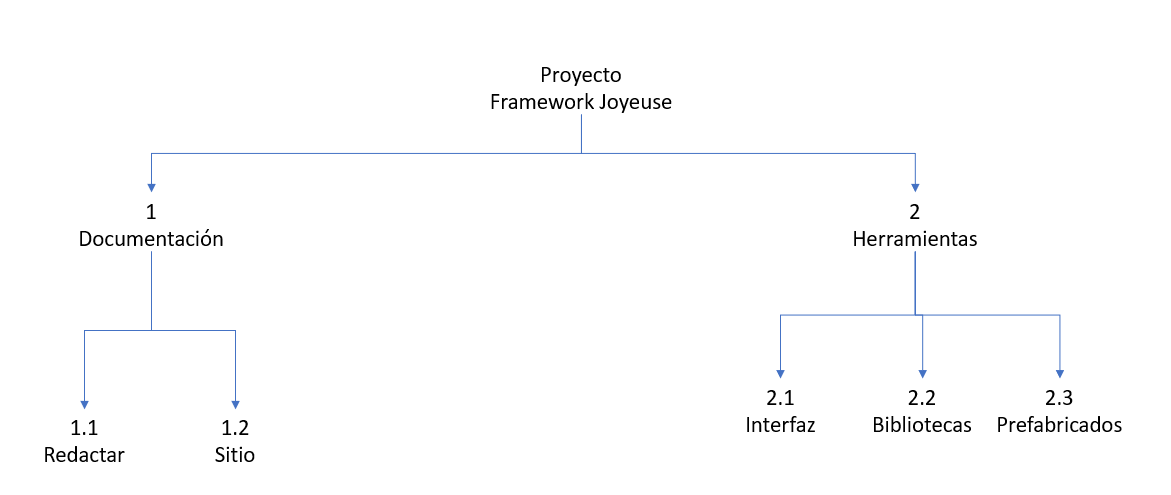
\includegraphics[width=1\textwidth]{EDT}
	\caption{Estructura de desglose de trabajo.} 
	\label{EDT}
	
\end{figure}

%\begin{figure}[H]
%	\centering
%	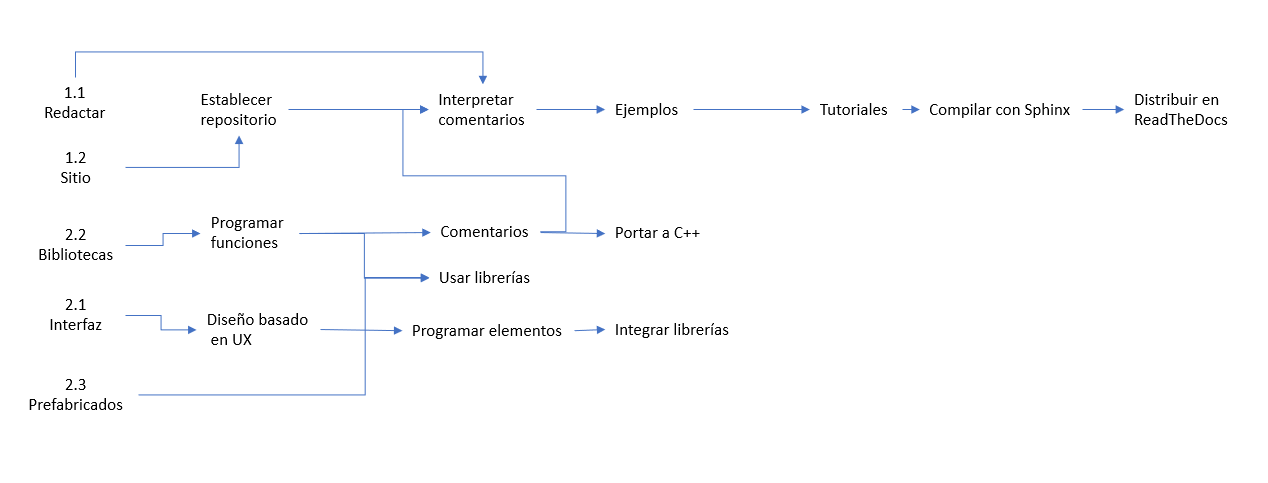
\includegraphics[width=1\textwidth]{EDT2}
%	\caption{Estructura de desglose de trabajo, actividades.}	
%\end{figure}

\section{El Framework}


\subsection{Prop\'osito}

Acelerar el desarrollo 
de videojuegos al permitir a los desarrolladores 
enfocarse en los elementos que vuelven \'unicos a sus
juegos en vez de gastar tiempo en componentes b\'asicos comunes en la industria, adem\'as de facilitar el inicio del desarrollo y aprendizaje para aquellos con nulo conocimiento sobre el tema, ya que le permite crear videojuegos sin temor a encontrarse barreras de c\'odigo a todo aquel que lo desee, acrecentando de esta forma la innovaci\'on creativa en la industria.

\subsection{Importancia}

Al cumplir la doble funci\'on de ser un software R.A.D. (Rapid Application Development) y un Framework, cubre dos campos interrelacionados de la industria que han sido descuidados a trav\'es del tiempo, en cuanto a Shooters respecta. 
Software que funciona con los mismos principios ha quedado obsoleto y olvidado, dejando un hueco que el software existente no podr\'ia llenar debido a su nivel de complejidad.
\newline
Es necesario mencionar el por qu\'e de las decisiones respecto a la orientaci\'on del proyecto: los Shooters acaparar\'an m\'as de 25.9\% del  mercado americano de los v\'ideo juegos para el a\~no 2019, seg\'un la proyecci\'on basada en la figura~\ref{fig:FORB}  y la figura~\ref{fig:STAT} de la p\'agina~\pageref{fig:STAT}.


\begin{figure}[H]
	
	\centering
	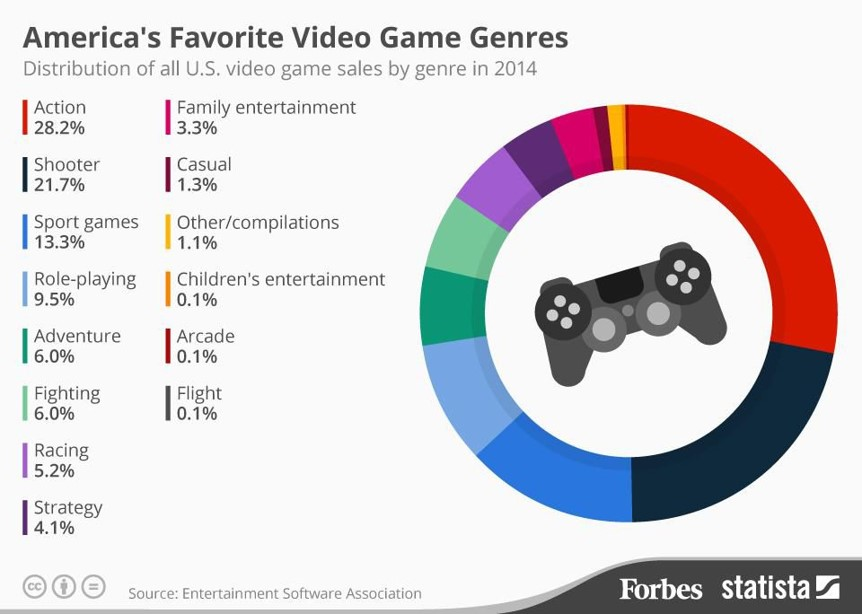
\includegraphics[width=0.5\textwidth]{Picture1}
	\caption{Cuota de mercado, por g\'enero, porcentajes del a\~no 2014.} 
	\label{fig:FORB}
	\cite{Forbes}
	
	
\end{figure}

\begin{figure}[H]
	
	\centering
	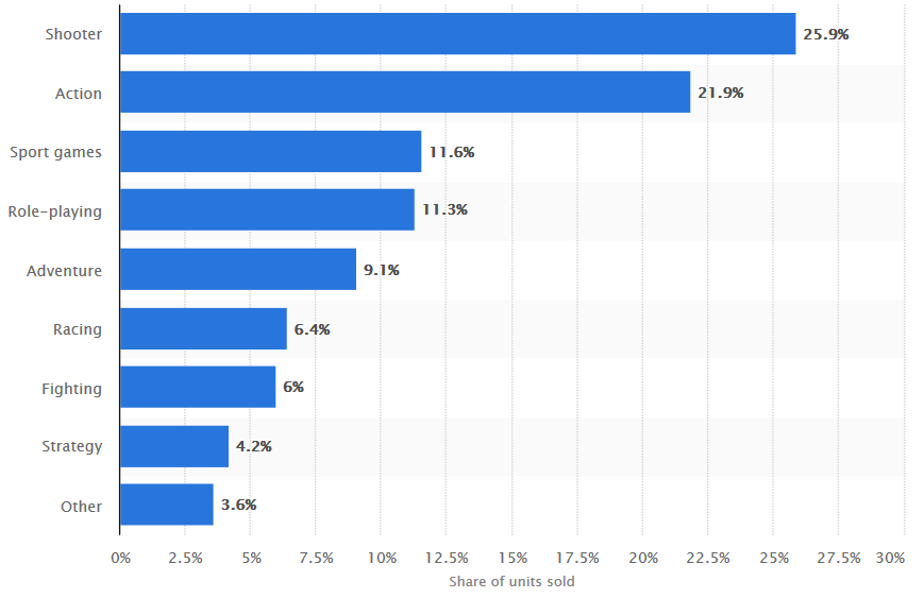
\includegraphics[width=0.5\textwidth]{statista-2}
	\caption{Cuota de mercado, por g\'enero, porcentajes del a\~no 2017.  } 
	\label{fig:STAT}
	\cite{Statista}
	
	
\end{figure}

 Estados Unidos es el segundo mayor cosumidor a nivel global, con ingresos de \$32.7 mil millones de d\'olares, tan solo \$7.5 mil millones debajo de China. 
 El motivo para elegir al mercado am\'ericano sobre al chino, es la libertad de publicaci\'on y contenido que existe en \'este; a diferencia de China, donde los videojuegos est\'an regulados por fuertes restricciones y filtros impuestos por el gobierno.
 %Añadir bibliografía

\begin{figure}[H]
	
	\centering
	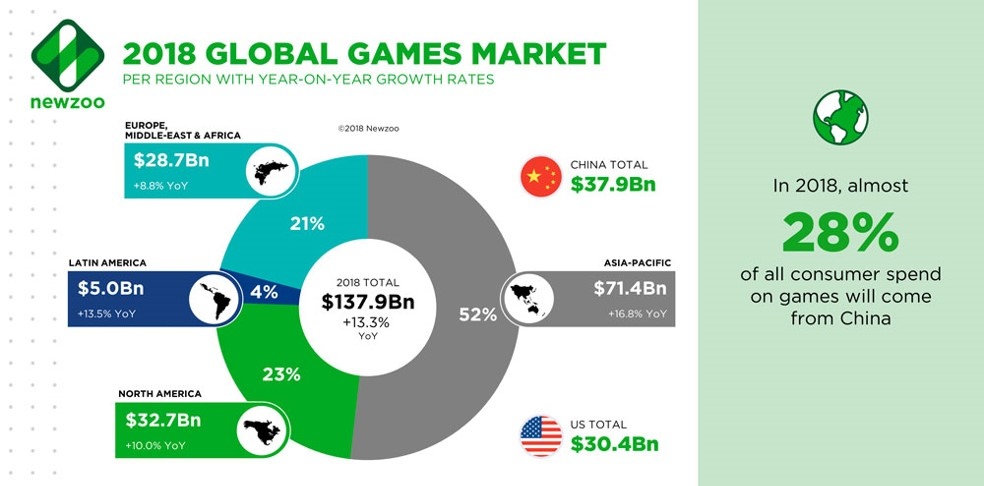
\includegraphics[width=1\textwidth]{GGM2}
	\caption{Procedencia de los ingresos anuales, 2018.  } \cite{Newzoo} 
	\label{NWZOO}
	
\end{figure}

Considerando los puntos anteriores, es posible calcular la proyecci\'on de ingresos para los shooters en el a\~no 2019: considerando las tazas de crecimiento anual, podemos esperar un aumento del 6.45\% en la cuota de mercado, lo que se traduce en 9.54 mil millones de d\'olares en ganancias. 

\subsection{Impacto}
Como principal impacto, adem\'as del econ\'onmico, para el cual se posee un amplio repertorio de posibilidades, la educacion recibir\'ia un apoyo sustancial, ya que se conseguir\'ia acercar a la programaci\'on a cualquier persona con acceso a una computadora. Por otro lado cabe destacar que se lograr\'ia revivir un sector de la industria cuya oferta decay\'o en a\~nos recientes y que a\'un tiene demanda. Dar una herramienta de este tipo para su uso libre, sin l\'imites para el usuario, ya sean estos de tipo comercial, legal o estructural, permitir\'a el nacimiento de juegos m\'as diversos, ya que se borrar\'a la barrera entre desarrolladores, artistas y jugadores.


\subsection{Trabajo relacionado}

\subsubsection{Entidad 3d}

Creado en el 2004, tuvo un cese del desarrollo entre 2008 a 2013, para ser abandonado finalmente por el creador en 2016. La cantidad de diferentes enemigos, armas, personajes y din\'amicas es limitada. Utiliza niveles BSP (Partici\'on Binaria del Espacio), los cuales limitan el motor a crear juegos en habitaciones y pasillos y exteriores peque\~nos. 

Es incompatible con Windows 8 y presenta problemas de compatibilidad con Windows 10, ya que varios paquetes que utilizaba, como DirectPlay, dejaron de ser activados por defecto desde Windows 7. 


El punto fuerte del motor es su documentaci\'on extensiva, llena de ejemplos pr\'acticos.
Utiliza DirectX8 y OpenGL 1 para renderizar las escenas.
Su c\'odigo es cerrado, lo que significa que jam\'as volver\'a a recibir una actualizaci\'on.


\subsubsection{GameGuru}

El motor fue creado en el 2012 como sucesor de FPSCreator y a pesar de que el desarrollo est\'a detenido, a\'un recibe mantenimiento y contenido. 
Utiliza LUA como lenguaje de scripts (\#20 en PYPL).
La API gr\'afica que utiliza DirectX11, disponible únicamente en Windows. Otorga la posibilidad de usar modelos y texturas propios, vendi\'endolos tambi\'en como contenido descargable. Se encuentra disponible para ser comprado, bajo c\'odigo cerrado.

\subsubsection{FPS Creator}

Fue lanzado en 2005, con gr\'aficos DirectX9, su \'ultima actualizaci\'on fue en el 2017 a trav\'es de un mod creado por la comunidad llamado "Black Ice Mod", sin embargo, el multijugador llevaba sin soporte desde el 2015. \cite{MP_discontinued}

El motor estaba l\'imitado a un uso m\'aximo de RAM de 2GB al momento de la compilaci\'on, lo que se traduce en un m\'aximo de 5 niveles por juego.
S\'olo disponible para Windows.
Actualmente su c\'odigo est\'a alojado en Github, sin una licencia especificada, lo cual deja al motor y posibles modificaciones en ambig\"uedad legal. 


\subsubsection{SilentWalk FPS}

Creado en el 2008, recibi\'o s\'olo una actualizaci\'on antes de que parase el desarollo. El nivel de usuarios fue bajo desde siempre e incluso aunque la comunidad sigue existiendo, el sitio oficial dej\'o de tener el enlace a esta desde mayo del 2018. 
Utiliz\'o DirectX 9 en el apartado gr\'afico, su c\'odigo permanece cerrado. 

\subsubsection{Reality Factory}

Fue publicado inicialmente en 2006 y recibi\'o su \'ultima actualizaci\'on en el a\~no 2014. Utiliza DirectX9 para los gr\'aficos. La estructura de niveles es BSP y utiliza Simkin como lenguaje de scripts, incluye las herramientas necesarias para crear personajes, objetos, di\'alogos y texturas, tambi\'en incluye modelos, sonidos y texturas para crear prototipos. Da la opci\'on de cambiar entre c\'amara en primera y tercera persona. De c\'odigo abierto.


\subsection{Patentes relacionadas}

\subsubsection{Game production tool supporting multi platform using game development tool}

\paragraph{Resumen}
La presente invenci\'on se refiere a una herramienta de producci\'on de juegos que soporta una plataforma m\'ultiple que usa una herramienta de desarrollo de juegos. De acuerdo con la presente invenci\'on, un art\'iculo, una persona y un fondo que aparecen en un espacio virtual en un juego se definen como objetos del juego y un estado en el que los objetos del juego se muestran en una pantalla en el espacio virtual se genera en forma de M\'ultiples cuadros de imagen se muestran secuencialmente en la pantalla. La presente invenci\'on incluye una unidad de entrada de datos en la que un usuario ingresa datos del juego que incluyen un objeto del juego, dise\~no del juego, planificación del juego y un gui\'on del juego, un módulo personalizado de datos de entrada del usuario que incluye una unidad de conversi\'on de datos que convierte la entrada de datos ingresados en el juego a datos optimizados para la herramienta de desarrollo del juego, un m\'odulo de elementos de la colecci\'on de eventos que genera m\'ultiples listas de eventos que pueden ocurrir durante un juego al analizar los datos optimizados transmitidos desde la unidad de conversi\'on de datos, y un cliente del juego en el que un usuario designa el orden de las m\'ultiples listas de escenas de eventos generadas en el m\'odulo de elementos de la colecci\'on de escenas de eventos para su aplicaci\'on a la herramienta de desarrollo del juego.
\cite{multip}
\paragraph{Comparativa}
Joyeuse, al igual que el programa de la patente, toma informaci\'on a trav\'es de la interacci\'on de un usuario con una interf\'az intuitiva, parecida a un juego, para despu\'es interpretarla para posibilitar que Godot compile el juego. Sin embargo no utiliza un sistema de eventos posibles, se alienta al usuario a crear sus propios eventos a trav\'es del sistema de comandos. 
\subsubsection{Visual game level editing method and system based on trigger}
\paragraph{Resumen}
La invenci\'on describe un m\'etodo y sistema de edici\'on visual a nivel de juego basado en un activador, en el que el m\'etodo comprende los siguientes pasos de 
\newline
\newline A, acceso a una base de datos de desarrollo de juego y actualizaci\'on y obtenci\'on de recursos y datos de dise\~no a nivel de juego; 
\newline
\newline B, que proporciona una interfaz de interacci\'on hombre-computadora, en donde la interfaz de interacci\'on hombre-computadora comprende una regi\'on de edici\'on de estratagema, una regi\'on de edici\'on de nivel y una regi\'on de actividad de configuraci\'on de par\'ametros; 
\newline
\newline
C, carga los recursos de dise\~no a nivel de juego y los datos en elementos en la regi\'on de edici\'on de estratagema y la regi\'on de edici\'on de nivel configurada por un usuario, y traduce al menos un elemento de combinaci\'on de estratagema probado en un archivo de formato de datos de nivel y transmite el archivo de formato de datos de nivel a Una herramienta de edici\'on de nivel de juego para crear o actualizar el nivel. \newline 
\newline El sistema comprende un primer m\'odulo, un segundo m\'odulo y un tercer m\'odulo, en donde el primer m\'odulo se usa para acceder a la base de datos de desarrollo del juego; el segundo m\'odulo se utiliza para proporcionar la interfaz de interacci\'on hombre-computadora; y el tercer m\'odulo se utiliza para exportar el archivo de formato de datos de nivel. El m\'etodo y el sistema tienen las ventajas de que el costo de desarrollo a nivel del juego se reduce obviamente; Se ha mejorado la reutilizaci\'on y la mantenibilidad del c\'odigo.
\cite{leveledit}
\paragraph{Comparativa}

Similar a la forma en la que Joyeuse maneja los ficheros y la interacci\'on proporcionada por el usuario, siendo un paquete comprimido de formato .pck el que cumple la funci\'on de la base de datos. En el caso de Joyeuse, se provee un editor de niveles que se comunica directamente con el motor, guardando la informaci\'on en formato nativo, por lo que no se requiere traducci\'on de datos o formato. 





\subsubsection{Server synchronization graph handle tools}
\paragraph{Resumen} 
La presente invenci\'on se refiere a un m\'etodo para producir contenidos de juegos. Para esto, en la presente invenci\'on, mediante el uso de una herramienta de producci\'on de manejador gr\'afico, se produce un nuevo patr\'on combinando muchos patrones que ya se han producido. Al repetir este proceso, un operador que ha aprendido a usar la herramienta de producci\'on de manejadores gr\'aficos puede revisar y producir f\'acilmente nuevos contenidos sin conocimiento profesional sobre el desarrollo de un juego, y puede extraer el script. Por lo tanto, la presente invenci\'on hace que el mantenimiento sea conveniente.
\cite{Server}
\paragraph{Comparativa}
Tanto el proyecto como esta patente buscan ofrecer la capacidad de producir videojuegos sin tener conocimientos profesionales, sin embargo la patente en cuesti\'on se enfoca a la producci\'on de contenido a trav\'es de patrones y la sincronizaci\'on de los servidores. 














\subsubsection{Tool for video game application development}
\paragraph{Resumen} 
Se describen t\'ecnicas que pueden modificar el contenido de una aplicaci\'on de videojuegos que se ejecuta en una plataforma de juegos. La t\'ecnica incluye el acoplamiento comunicativo con la plataforma del juego para intercambiar mensajes con la plataforma del juego. Una herramienta puede recibir datos representativos de una versi\'on de una pantalla representada por la plataforma del juego. La herramienta puede luego presentar su propia versi\'on de la pantalla y modificar los datos de contenido que conforman la imagen de la pantalla. La herramienta puede enviar un mensaje de modificaci\'on de contenido a la plataforma del juego, el mensaje incluye datos representativos de las modificaciones realizadas por la herramienta. La plataforma del juego puede modificar y generar una nueva versi\'on de la pantalla en la plataforma del juego seg\'un el mensaje de modificaci\'on.
\cite{EA}
\paragraph{Comparativa}
La patente se enfoca en describir un m\'etodo para la comunicaci\'on entre una interf\'az y una plataforma de v\'ideojuegos, para modificar esta misma, enfoc\'andose en la sincronizaci\'on entre la plataforma y el juego en s\'i, no en la creaci\'ona diferencia de Joyeuse que genera y modifica contenido sin depender de una plataforma. 
\subsubsection{Educational game engine capable of directly developing and combining content}
\paragraph{Resumen} 
PROP\'OSITO: se proporciona un motor de juego educativo para implementar f\'acilmente la combinaci\'on de motores y el desarrollo de contenido de un usuario mediante m\'odulos de funciones en una interfaz de programa de aplicaci\'on. 
\newline
\newline
CONSTITUCI\'ON: Un motor de juego educativo incluye una interfaz de programa de aplicaci\'on en un m\'odulo de funci\'on para combinar un motor de juego educativo y un m\'odulo de funci\'on. El motor de juegos educativo es presentado con el lenguaje inform\'atico C ++ que es de f\'acil acceso para un usuario. La interfaz del programa de la aplicaci\'on se configura en base a una tecnolog\'ia orientada a objetos. La interfaz del programa de aplicaci\'on reemplaza un m\'odulo de funci\'on con un m\'odulo de funci\'on de creaci\'on de usuario.
\cite{Edu}
\paragraph{Comparativa}
En este caso, se comparte uno de los objetivos del Framework en el \'ambito educativo, sin embargo en Joyeuse se prefiere utilizar un sistema de comandos interpretados que se asemeje a la escritura de un texto o pseudo-c\'odigo, o en su defecto un sistema de programaci\'on visual a trav\'es de nodos. 

\subsection{Diagrama de Flujo de Datos}
\begin{figure}[H]
	
	\centering
	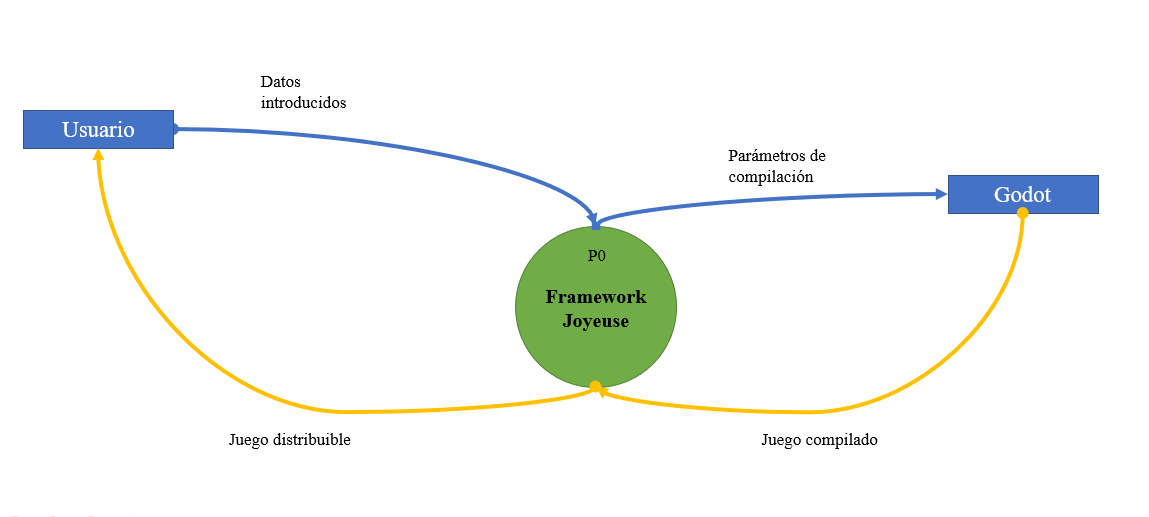
\includegraphics[width=1\textwidth]{DFD}
	\caption{Diagrama de contexto (Nivel 0).} 
	\label{DFD0}
	
\end{figure}
\begin{figure}[H]
	
	\centering
	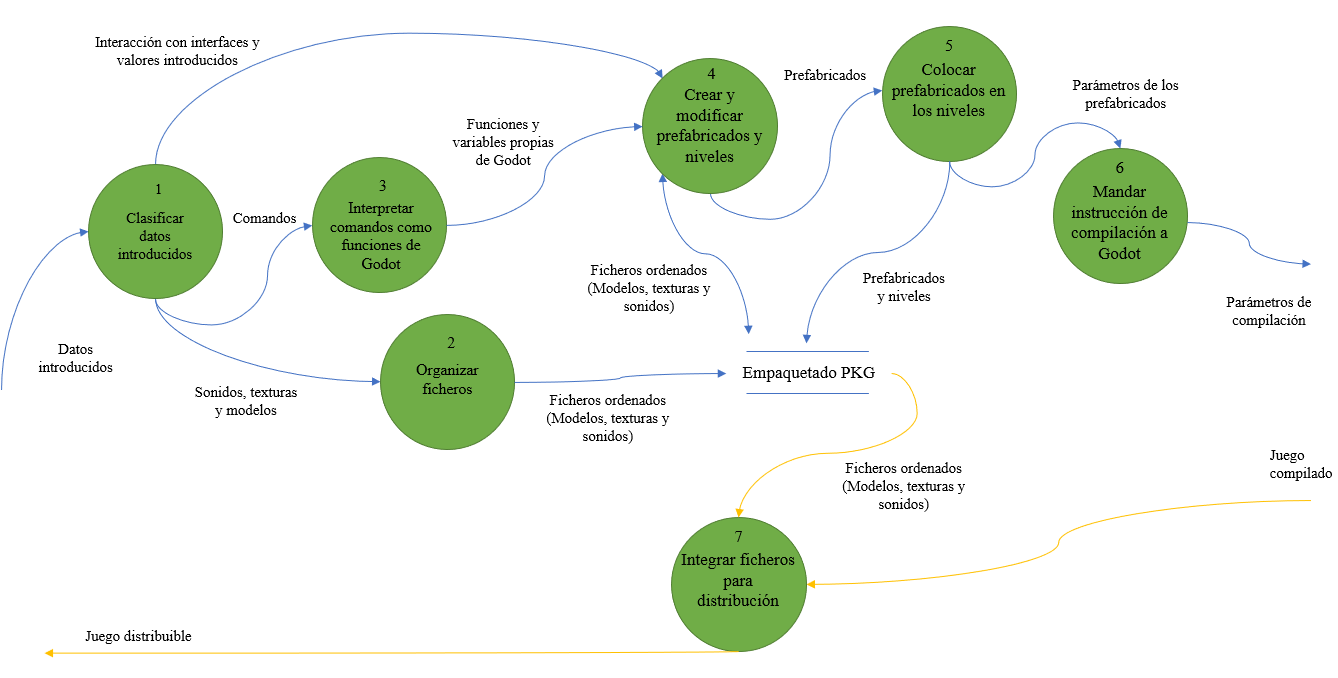
\includegraphics[width=1\textwidth]{DFD2}
	\caption{Diagrama de Flujo de Datos, Nivel 1.} 
	\label{DFD1}
	
\end{figure}




  



\newpage
\bibliography{Joyeuse}
\bibliographystyle{APA}



\end{document}